% Teilaufgabe 3

\section{Dunkelfeldmikroskop in Transmission}
\label{sec:mikroskop}

\subsection{Aufbau und Funktionsweise}
\label{sub:aufbau}

\begin{center}
    \captionsetup{type = figure}
    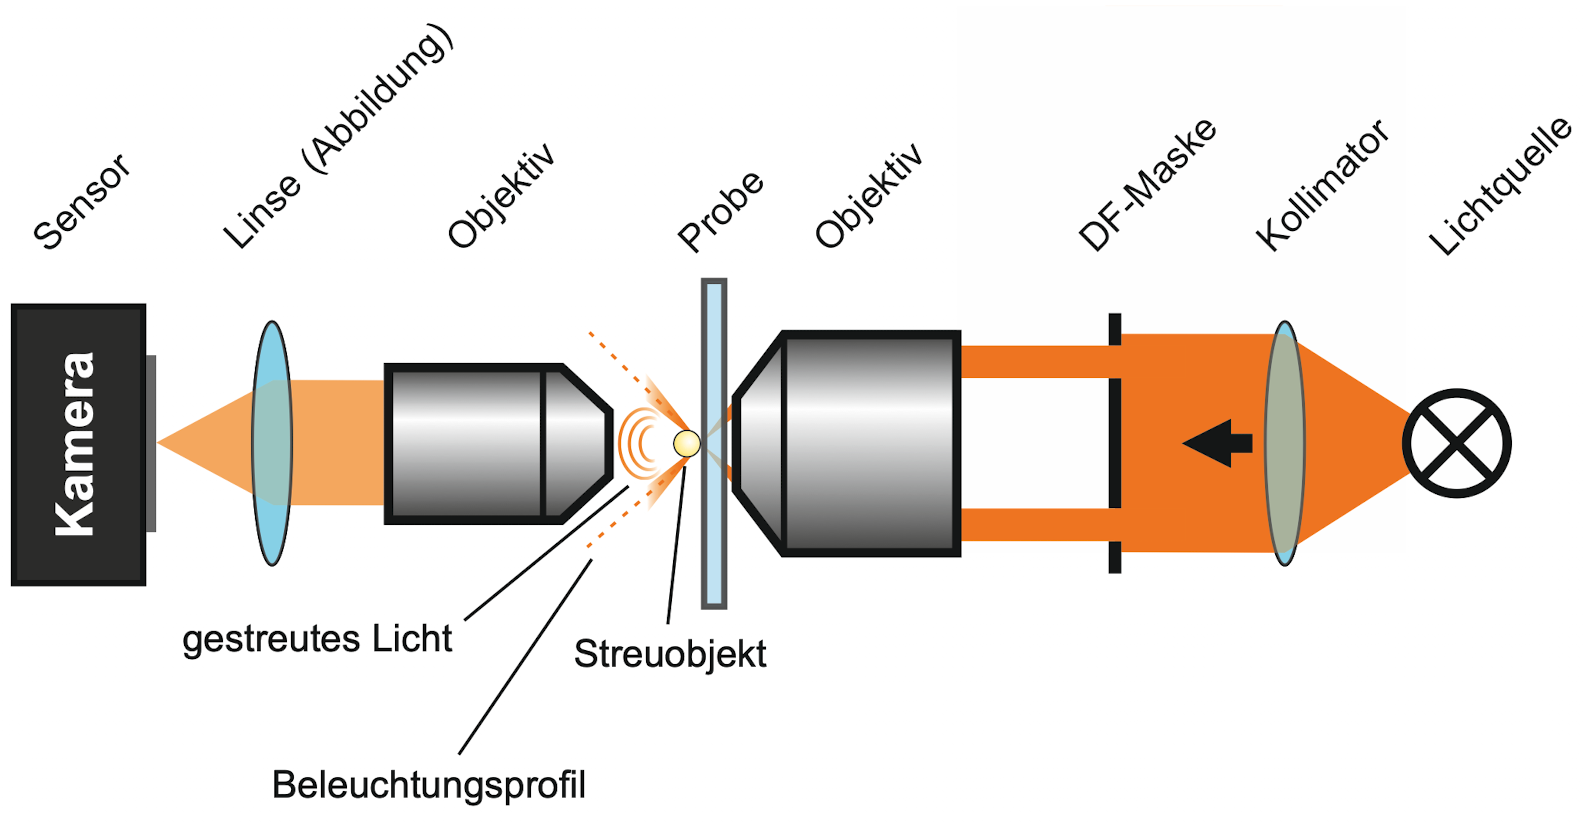
\includegraphics[width = 0.9\textwidth]{Bilder/Aufbau_Dunkelfeld.png}
    \captionof{figure}{Einfacher Aufbau eines Dunkelfeldmikroskops in Transmission. Eine breitbandige Lichtquelle wird mittels einer Optik kollimiert. Eine Maske (DF-Maske) schneidet einen Ring in das Strahlprofil. Der so geformte Strahl wird mittels Objektiv auf die Probe fokussiert. Ein weiteres Objektiv sammelt das von der Probenoberfläche bzw. dem Objekt gestreute Licht auf, wodurch kein direktes Licht der Beleuchtung eingesammelt wird. Das gestreute Licht wird über eine Linse auf den Kamerasensor abgebildet. \cite{Anleitung}}
    \label{fig:aufbau}
\end{center}

Die Dunkelfeldmikroskopie ist eine hintergrundfreie Methode, was bedeutet, dass kein Hintergrundsignal detektiert wird, sondern nur Informationen von dem untersuchten Objekten. In Abb. \ref{fig:aufbau} ist der schematische Aufbau des Dunkelfeldmikroskops in Transimission abgebildet. Auf der rechten Seite steht die Lichtquelle, die mittels einer Linse kollimiert wird. Dahinter befindet sich eine inverse Lochblende (DF-Maske), die lediglich die Ränder des Lichtkegels transmittiert. Mit einem Objektiv relativ hoher numerischer Apertur wird die Probe beleuchtet, wobei auf der anderen Seite der Probe befindet sich ein Objektiv mit geringerer numerischer Apertur. Durch diese besondere Beleuchtung kann kein direktes Erregerlicht in dieses Objektiv fallen, wodurch die Abbildung der Probenoberfläche auf der Kamera dunkel erscheint. Befindet sich jedoch ein Streukörper, zum Beispiel ein Nanopartikel, auf der Probenoberfläche so wird das Erregerlicht daran gestreut, was widerum vom Objektiv aufgesammelt und detektiert werden kann. \cite{Anleitung}

\subsection{Messung von plasmonischen Eigenschaften}
\label{sub:messungEigenschaften}

Das Prinzip der Dunkelfeldmikroskopie beruht darauf, dass Objekte Licht nicht nur absorbieren, sondern auch immer einen Teil des Lichtstrahls ablenken. Die Stärke eines Signals ist bei der Dunkelfeldmikroskopie nicht von der Größe einer Struktur abhängig, sondern davon wie stark das Licht von ihr abgelenkt wird. Eine der Ablenkungsursachen ist die als Tyndall-Effekt bezeichnete Streuung von Licht an kleinen Teilchen, welche beispielsweise auch zu beobachten ist, wenn Licht in einen dunklen Raum fällt und der Staub innerhalb des Lichtstrahls deutlich sichtbar wird. Daher können auch Partikel oder Strukturen nachgewiesen werden, die kleiner sind als die Auflösungsgrenze des jeweiligen Mikroskops. \cite{WikiDunkelfeld}

\subsection{Hintergrundkorrigiertes Dunkelfeldspektrum}
\label{sub:korrigiertesSignal}

In diesem Versuch wird zusätzlich zum hintergrundfreien Streuspektrum der Partikel auch noch das Lampenspektrum der Beleuchtungseinheit, sowie ein Spektrum ohne Beleuchtung aufgenommen. Um ein hintergrundkorrigiertes Dunkelfeldspektrum zu erhalten, wird im folgenden vom Lampenspektrum das Spektrum ohne Beleuchtung abgezogen, was im weiteren als effektives Lampenspektrum bezeichnet wird. Das effektive Lampenspektrum wird wiederum vom Streuspektrum des Partikels abgezogen, wobei hier auch das Spektrum ohne Beleuchtung abgezogen wurde. Nach dieser Argumentation wird klar, dass beide Spektren (Lampenspektrum und Streuspektrum) den gleichen Hintergrund Offset (Spektrum ohne Beleuchtung) teilen. Weshalb vorgeschlagen wird die Korrketur, um den Offset zu vernachlässigen und nur um das Lampenspektrum zu korrigieren. 